%\documentclass{article}
%a4paper,landscape
\documentclass[aps,reprint,floatfix]{revtex4-1}
%\setlength{\parindent}{0pt}
\newcommand{\forceindent}{\leavevmode{\parindent=1em\indent}}
%\usepackage{graphicx}
\usepackage{comment}
%\usepackage{biblatex}
\usepackage{hhline}
\usepackage{float}
\usepackage{tabularx}
\usepackage{tikz}
\usepackage{pgfplots}
\pgfplotsset{width=7cm,compat=1.3}
%\pgfplotsset{width=13cm,compat=1.9}
\usepackage{circuitikz}
\usepackage{tikz}

\usepackage{graphicx}
\usepackage{placeins}
\usepackage{amsmath}
%\newcommand{\Mod}[1]{\ (\mathrm{mod}\ #1)}
%\newcommand{\backup}{\vspace{-0mm}}

\begin{document}

\begin{titlepage}
	\centering
	
\includegraphics[width=0.15\textwidth]{CHSLogo.png}\par\vspace{1cm}
	{\scshape\LARGE Charlottesville High School \par}
	\vspace{1cm}
	{\scshape\Large AP Physics C Lab 05\par}
	\vspace{1.5cm}
	{\huge\bfseries An Unparalleled Examination of a Series of Kirchoff's Rules \par}
	\vspace{2cm}
	{\Large\itshape Jack Timmins \par}
	\vspace{9.75cm}
	supervised by\par
	Prof.~Stephen Newman\par
	March 13rd 2018
	\newpage
\end{titlepage}

\section{Abstract}
\forceindent Resistance is a property of a material that is defined, in sensible materials, as $\frac{V}{I}$. It is a hindrance to current and releases energy, via heat, to provide a drop in voltage. This series — or parallel — of experiments are aimed at confirming Kirchhoff's rules for circuits.

\section{Notation}

$R_{eq}$: Combined resistance of one or more resistors

\section{Introduction}
	
	\subsection{General Analysis}	
		
	\forceindent Kirchoff's rules provide a framework for understanding circuits and they are as follows: all voltage gains equal voltage drops in a circuit, loop rule, and the sum of currents entering a node exit equal to the sum of currents exiting a node, nodal rule:
	
	\begin{equation}
		\sum_{k=1}^{n} V_k = 0
		\label{An example of the 1st rule}
	\end{equation}
	
	\begin{equation}
		\sum_{in=1}^{n} I_{in} = \sum_{out=1}^{n} I_{out}
		\label{An example of the 2nd rule}
	\end{equation}

	\forceindent Combined with Ohm's law, $V = I R$, these can be used to derive expressions for find $R_{eq}$ for resistors in series and in parallel:
	
	\subsection{Resistors in Series}
	\forceindent The following is a proof for finding $R_{eq}$ for a circuit containing two resistors, $R_1$ and $R_2$, wired in series to a battery with voltage $V$. Since the resistors are in series they have the same current going through them.

	\begin{figure}[h]
	\begin{circuitikz}
	\draw
		(0,0)	to[battery, l=$V$, i=$I$]		(0,2)
				to[resistor, l=$R_1$]	(4,2) -- (4,0)
      			to[resistor, l=$R_2$] 	(0,0)
	;
	\end{circuitikz}
	\end{figure}
	
	Define $R_{eq}$
	$$ \frac{V}{I} = R_{eq} $$
	Apply the loop rule	
	$$ V = R_1 I + R_2 I $$
	Solve for $\frac{V}{I}$
	$$ \frac{V}{I} = R_1 + R_2 $$
	Giving
	\begin{equation}
		R_{eq} = R_1 + R_2
	\end{equation}
	
	\subsection{Resistors in Parallel}
	\forceindent The following is a proof for finding $R_{eq}$ for a circuit containing two resistors, $R_1$ and $R_2$, wired parallel to a bettery with voltage $V$. Since the resistors are in parallel they have the same potential difference $V$. 
	
	\begin{figure}[h]
	\begin{circuitikz}
	\draw
		(0,0)	to[battery, l=$V$, i=$I$]		(0,2.75) -- (2,2.75)
				to[resistor, l=$R_1$, i=$I_1$]	(2,0) -- (0,0)
		(2,2.75) -- (4,2.75)
				to[resistor, l=$R_2$, i=$I_2$]	(4,0) -- (2,0)
	;
	\end{circuitikz}
	\end{figure}
	
	Define $R_{eq}$	
	$$ \frac{V}{I} = R_{eq} $$
	Apply the node rule
	$$ I_0 = I_1 + I_2 $$
	Apply Ohm's law
	$$ \frac{V}{R_{eq}} = \frac{V}{R_1} + \frac{V}{R_2} $$
	Solve for $R_{eq}$ gives
	\begin{equation}
		R_{eq} = \bigg( \frac{1}{R_1} + \frac{1}{R_2} \bigg) ^{-1}
	\end{equation}

\section{Experiments}

	\subsection{Error}
	\forceindent For the measurements in all of our experiments, we used an ohmmeter with 1\% error. For our percent error calculation we used the following formula: 
		\begin{equation}
			\sigma_f = \sqrt{ \bigg( \frac{\partial f}{\partial a_0} \sigma_{a_0} \bigg) ^ 2 + \bigg( \frac{\partial f}{\partial a_1} \sigma_{a_1} \bigg) ^ 2 + ... + \bigg( \frac{\partial f}{\partial a_n} \sigma_{a_n} \bigg) ^ 2 }
		\end{equation}

\subsection{Resistors in Series}
\forceindent In this experiment, we attempt to verify our prediction about the $R_{eq}$ of resistors wired in series. In order to do this, we retrieve two nominal $220 \Omega$ resistors, marking one to make them distinguishable, and measure them both with our digital ohmmeter. We then wire both resistors in series and measure them yielding $435 \pm 14.35 \Omega$. Using Eqn. (3), we find that our experimental value fell within $0.17 \sigma$ from our predicted value. We conclude that our data provides evidence for the formula derived for finding the $R_{eq}$ of resistors wired in series.

\begin{table}[h]
	%\centering
	\begin{tabular}{|c||c|c|}
		\hline		
		Label: 				& Resistance (in $\Omega$):\\ 
		\hline
		\hline
		Resistor \#1			& $215.00 \pm 12.15$ \\ \hline
		Resistor \#2			& $217.00 \pm 12.17$ \\ \hline
		Measured $R_{eq}$		& $432.00 \pm 17.20$ \\ \hline
		Theoretical $R_{eq}$	& $435.00 \pm 14.35$ \\
		\hline
	\end{tabular}
\caption{Results of Experiment B.}
\end{table}

\subsection{Resistors in Parallel}
\forceindent In this next experiment, we test the derived formula for finding the $R_{eq}$ of resistors wired in parallel. We acquire two nominal $10$k$\Omega$ resistors, marking one to make them distinguishable, and measure their resistance individually labeling them A and B with our digital ohmmeter. After measuring, we wire them in parallel and measure them yielding $4850.00 \pm 148.5$k$\Omega$. Using Eqn. (4), we conclude that because our experimental value fell within $0.0 \sigma$ away from my predicted value, our data supports confirms our derived formula for the $R_{eq}$ of resistors in parallel.

\begin{table}[h]
	%\centering
	\begin{tabular}{|c||c|c|}
		\hline		
		Label: 				& Resistance (in $\Omega$):\\ 
		\hline
		\hline
		Resistor A				& $9700.00 \pm 197.00$ \\ \hline
		Resistor B				& $9720.00 \pm 197.20$ \\ \hline
		Measured $R_{eq}$		& $4850.00 \pm 69.69$ \\ \hline
		Theoretical $R_{eq}$	& $4850.00 \pm 148.50$ \\
		\hline
	\end{tabular}
\caption{Results of Experiment C.}
\end{table}

\subsection{Multiple Resistors in Parallel}
\forceindent In this final experiment, we retest the derived formula for resistors wired in parallel. We retrieve eight additional nominal $220 \Omega$ resistors, reusing the resistors used in experiment B, and measure / marke them individually to obtain a total of ten nominal $220 \Omega$ resistors, labeling them 1-10 respectively. We then wire resistors 1 and 2 in parallel, measure them, and label the result trial 1. We then wire resistor 3 to trial 1’s configuration in parallel and measure it labelling it trial 2. We continue adding one resistor at a time and increment trials until we have ten resistors wired in parallel and it is labelled trial 9. Displayed in FIG. 1, against theoretical values found using Eqn. (4), we find more evidence supporting our derived formula for $R_{eq}$ of resistors measured in parallel.

\begin{table}[h]
	\begin{tabular}{|c||c|c|}
		\hline		
		Label: 				& Resistance (in $\Omega$):\\ 
		\hline
		\hline
Resistance of 220Ω \# 1	&	$	215.00	\pm	12.15	$	\\	\hline
Resistance of 220Ω \# 2	&	$	217.00	\pm	12.17	$	\\	\hline
Resistance of 220Ω \# 3	&	$	215.00	\pm	12.15	$	\\	\hline
Resistance of 220Ω \# 4	&	$	214.00	\pm	12.14	$	\\	\hline
Resistance of 220Ω \# 5	&	$	214.00	\pm	12.14	$	\\	\hline
Resistance of 220Ω \# 6	&	$	213.00	\pm	12.13	$	\\	\hline
Resistance of 220Ω \# 7	&	$	216.00	\pm	12.16	$	\\	\hline
Resistance of 220Ω \# 8	&	$	216.00	\pm	12.16	$	\\	\hline
Resistance of 220Ω \# 9	&	$	219.00	\pm	12.19	$	\\	\hline
Resistance of 220Ω \# 10&	$	217.00	\pm	12.17	$	\\	\hline
	\end{tabular}
\caption{Results of Experiment C.}
\end{table}

\begin{figure}[h]
	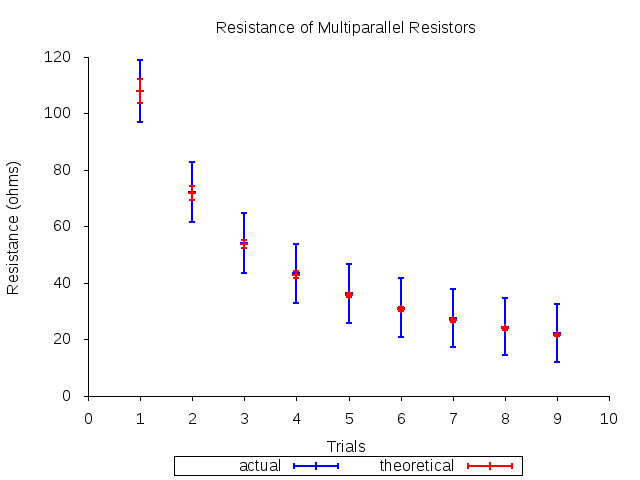
\includegraphics[scale=.53]{resistor.png}
	\caption{Results of Experiment C.}
\end{figure}

\section{Conclusion}
In this report, we observed the $R_{eq}$ of resistors wired in series and in parallel wired to an ohmmeter. The measured $R_{eq}$ was found, in both cases, to confirm our predictions. We confirm that Kirchhoff's rules regarding circuits can be used to accurately predict $R_{eq}$ of a circuit with resistors. Additionally, we find that in order to most accurately measure resistance in series resistors they should be measured once wired and to most accurately measure resistance in parallel they should be measured individually predicted using Kirchoff's rules.

\end{document}